\documentclass[10pt]{article} % For LaTeX2e
\usepackage{tmlr}
% Double-blind TMLR submission: no class option, so tmlr.sty replaces the
% author block with "Anonymous authors" and prints the "Under review" banner.
% The author block is anonymised in the source as well, so that submitting the
% LaTeX source cannot deanonymise the paper. Restore main_preprint.tex for the
% camera-ready. The Elsevier-style Declarations / Use of Generative AI / Data
% Availability block is deliberately absent here: TMLR does not use it, the
% Broader Impact Statement covers what it covered, and availability is stated
% anonymously in Section~3.9.

\input{math_commands.tex}

\usepackage{hyperref}
\usepackage{url}
\usepackage{graphicx}
\usepackage{booktabs}
\usepackage{amsmath}
\usepackage{amssymb}

\title{Decodable but Directionally Misaligned: Auditing Distance-Based OOD Ranking on Domain-Adversarial Skin-Lesion Representations}

\author{\name Anonymous authors \\ \addr Paper under double-blind review}

\hypersetup{
  pdftitle={Decodable but Directionally Misaligned: Auditing Distance-Based OOD Ranking on Domain-Adversarial Skin-Lesion Representations},
  pdfauthor={Anonymous},
  pdfsubject={Machine Learning, Trustworthy AI, Out-of-Distribution Detection},
  pdfkeywords={out-of-distribution detection, reliability estimation, representation geometry, disentanglement, domain-adversarial training, Mahalanobis distance, probing classifiers, distribution shift, trustworthy machine learning}
}

\begin{document}

\maketitle

\begin{abstract}
Distance-based out-of-distribution (OOD) scoring assumes not only that a learned representation separates source and shifted inputs, but also that the induced ordering has the correct operational direction: larger distance should indicate greater OOD likelihood. We audit this assumption within a domain-adversarial representation-learning regime using an orthogonality-strength ladder. Three checkpoint families share the same architecture and 16-dimensional representation and differ only in $\lambda_{\mathrm{orth}} = 0, 1, 5$. Covariance conditioning changed substantially across the ladder: the shared within-class covariance condition number increased by approximately two orders of magnitude (Kendall's $\tau = 0.84$, exact $p = 2.8 \times 10^{-5}$), whereas the other four geometry summaries tested showed no significant trend. Under the pre-specified higher-distance-is-more-OOD convention, Mahalanobis AUROC (ISIC-test vs.\ PAD-UFES) remained near 0.40 at every ladder level, and cosine-to-centroid and pooled $k$-nearest-neighbor scorers showed the same pattern. Reversing score orientation corresponds to an orientation-free separability of only 0.58--0.60, showing that the distances retain weak domain-separation signal but systematically rank PAD-UFES samples as more source-typical than ISIC-test samples. In contrast, supervised probes used only as existence tests recovered domain membership from the identical embeddings at 0.72--0.81 AUROC. The supported finding is therefore a scoped dissociation between domain decodability and the weak, directionally misaligned ordering imposed by the tested source-fitted distance rules. Power and bootstrap analyses show that the $n=13$ design can exclude only large monotonic associations; moderate effects remain unresolved. The finding neither shows that scalar distances contain no domain-separation signal nor establishes that domain-adversarial training or orthogonality regularization causes the misalignment.
\end{abstract}


\section{Introduction}
\label{sec:intro}

Deep neural networks are typically evaluated by predictive accuracy, yet deployment safety also depends on how a learned representation interfaces with downstream reliability mechanisms. A distance-based OOD score must satisfy two distinct requirements. First, it must retain some ability to separate source and shifted inputs. Second, that separation must have the correct operational orientation: under the usual distance convention, shifted inputs should receive larger scores. A score can therefore contain distribution-separation signal while remaining unusable as specified if it orders the two distributions in the wrong direction. What matters is not ``geometry'' in the undifferentiated sense, but the particular geometric structure and ordering to which a scoring functional is sensitive. Covariance conditioning, class separation, local neighborhoods, angular relationships, and distributional shape can move differently under training; a change in one of these properties need not imply a corresponding change in OOD score ordering.

Distance-based OOD estimators make this dependence explicit. Mahalanobis distance \citep{lee2018simple}, cosine-to-centroid distance, and non-parametric $k$-nearest-neighbor scoring \citep{sun2022knn} all read a test input's location relative to the training distribution, but they preserve different invariances and discard different aspects of representation structure. Moreover, AUROC depends only on score ordering: any strictly increasing transformation leaves AUROC unchanged, whereas reversing score orientation maps an AUROC $a$ to $1-a$. An AUROC below 0.5 is therefore not evidence that the scalar score contains no distribution-separation signal. It instead indicates that, under the stated positive-class and score-direction convention, the score ranks the two groups predominantly in the opposite direction. We consequently distinguish throughout between \emph{directed OOD AUROC}, evaluated under the pre-specified higher-distance-is-more-OOD convention, and \emph{orientation-free separability}, summarized descriptively as $\max(\mathrm{AUROC},1-\mathrm{AUROC})$. The latter is a diagnostic of separation, not a post-hoc corrected detector: a polarity chosen after observing evaluation labels cannot be claimed as an operational calibration.

Domain-adversarial representation learning \citep{ganin2015unsupervised, ganin2016domain} and orthogonality-based shared/private separation objectives \citep{bousmalis2016domain} provide a useful setting in which to audit this issue because they deliberately reorganize representation structure associated with nuisance variables such as acquisition site or imaging domain. We study an orthogonality-strength ladder within a domain-adversarial regime ($\lambda_{\mathrm{orth}}=0,1,5$), holding architecture and representation dimensionality fixed across its levels. The design supports statements about how measured quantities vary with orthogonality strength within this regime; because every checkpoint already belongs to the domain-adversarial regime and the available conventional baseline is not matched in architecture or dimensionality, it does not by itself identify either domain-adversarial training or orthogonality regularization as the cause of any observed OOD behavior.

Our audit separates four questions that are often conflated: (i) which measured aspects of representation structure vary across the orthogonality ladder; (ii) whether the directed OOD ranking produced by several distance-based scorers changes with those measured properties; (iii) whether the scalar scores retain any orientation-free domain separability; and (iv) whether domain membership remains recoverable from the full embeddings by a supervised reader. This separation prevents a below-chance directed AUROC from being misread as absence of information and prevents a label-informed score reversal from being presented as a deployable correction.

Across the ladder, covariance conditioning changes substantially while the other four geometry summaries tested show no significant trend. Five variants from three structurally distinct distance-based scorer families remain near 0.40--0.42 directed AUROC under the pre-specified OOD convention. Their corresponding orientation-free separability is only 0.58--0.60: the scores retain weak separation signal, but their ordering is systematically opposite to the intended operational direction. Supervised probes used as decodability existence tests recover substantially stronger domain membership information at 0.72--0.81 AUROC from the full embeddings. The central finding is therefore a scoped dissociation between domain decodability and the weak, directionally misaligned ordering delivered by the tested source-fitted distance rules within the audited domain-adversarial training regime, not a claim that distances contain no information and not a causal claim that disentanglement creates the misalignment.

\section{Related Work}
\label{sec:related-work}

Post-hoc OOD detectors are usually grouped by whether they read the classifier's output layer or its internal representation. Output-layer scores include maximum softmax probability \citep{hendrycks2017baseline}, ODIN \citep{liang2018enhancing}, energy-based scoring \citep{liu2020energy}, ReAct \citep{sun2021react}, ViM \citep{wang2022vim}, and activation shaping \citep{djurisic2023ash}; training-time objectives such as ELogitNorm \citep{ding2025enhancing} instead reshape representations so that such scores work better. Distance-based scorers read the penultimate representation directly: Mahalanobis distance \citep{lee2018simple}, pooled $k$-nearest-neighbor distance \citep{sun2022knn}, nearest-neighbor guidance \citep{park2023nnguide}, and Gram-matrix scoring \citep{sastry2020gram}. Benchmarking across this family \citep{yang2024oodsurvey, miyai2024generalized} compares detectors across architectures and datasets under a fixed training regime. We hold architecture and dataset fixed and ask the complementary question: whether one detector's behavior on one representation changes when that representation is deliberately reshaped by training.

Domain-adversarial training \citep{ganin2015unsupervised, ganin2016domain}, domain separation networks \citep{bousmalis2016domain}, correlation alignment \citep{sun2016coral}, and adversarial discriminative adaptation \citep{tzeng2017adversarial} all suppress a nuisance variable in the representation; disentangled representation learning \citep{higgins2017betavae, locatello2019challenging} pursues a related but distinct factorization. These methods are motivated by documented shortcut reliance in clinical imaging --- scanner and hospital artefacts in chest radiographs \citep{zech2018variable, degrave2021ai}, surgical skin markings in dermoscopy \citep{winkler2019association}, and above-chance accuracy on lesion-masked ISIC images \citep{bissoto2020debiasing} --- synthesized by \citet{geirhos2020shortcut}. They are evaluated by downstream accuracy, or by a discriminator's failure to recover the suppressed variable; to our knowledge, none is evaluated by whether a distance-based reliability estimator built on the resulting representation still behaves as it did before the intervention.

Probing measures what a frozen representation encodes \citep{alain2016understanding, hewitt2019designing}, with the standing caution that a successful probe does not show that the model itself uses the decoded information \citep{belinkov2022probing}; we use probes only in that restricted, existence-test sense. A separate line characterizes representation geometry directly --- intrinsic dimensionality \citep{levina2004maximum, facco2017estimating, ansuini2019intrinsic} and covariance conditioning --- and \citet{janiak2026geometry} report that such summaries track Mahalanobis-style detector performance across frozen foundation-model backbones. That association is measured between representations differing simultaneously in pretraining corpus, objective, architecture, and scale, so it does not establish what happens when the same geometric quantities are moved within one fixed representation by a specific training intervention.

Finally, predictive uncertainty is known to degrade under dataset shift \citep{ovadia2019can}, with consequences for clinical deployment \citep{finlayson2021clinician}. Skin-lesion OOD detection has been studied with deep isolation-forest scoring \citep{li2020deepif}, benchmarked across covariate-shifted and far-OOD regimes \citep{gutbrod2025openmibood}, and shown to leave classifiers overconfident \citep{pacheco2020outofdistribution}; skin tone is a distinct and largely orthogonal source of heterogeneity \citep{daneshjou2022disparities} that our dataset pair does not separate from acquisition-device shift (Section~\ref{sec:limitations}). That literature evaluates reliability estimators against naturally occurring shift, not against a representation that is itself the target of an explicit debiasing intervention. Calibration \citep{guo2017calibration}, selective prediction \citep{elyaniv2010foundations, geifman2017selective}, and conformal prediction \citep{angelopoulos2023conformal} are outside the scope evaluated here. Appendix~\ref{app:related-work} gives the extended treatment of all six adjacent literatures.

\section{Methods}
\label{sec:methods}

\subsection{Study design, data, and the orthogonality-strength ladder}
\label{sec:design}
\label{sec:datasets}
\label{sec:ladder}

For each of 13 checkpoints we extract $z_{\mathrm{lesion}}$ embeddings for the ISIC training set and for the ISIC-test/PAD-UFES evaluation split. From these embeddings we compute geometry metrics on the fitted Mahalanobis parameters (Section~\ref{sec:geometry-metrics}), score the evaluation split with three distance-based reliability estimators built on the identical embeddings (Section~\ref{sec:scorers}), and train three supervised probes on the same embeddings to quantify domain-information decodability independent of any distance-based scorer (Section~\ref{sec:probe}). Association between orthogonality strength, the measured representation summaries, reliability estimation, and decodability is then tested across the ladder using exact-permutation statistics (Section~\ref{sec:stats}). Figure~\ref{fig:study-design} in Appendix~\ref{app:methods} diagrams the pipeline.

The source domain is the ISIC 2019 training set \citep{codella2019skin, tschandl2018ham10000, combalia2019bcn20000} --- 25{,}331 images over the eight diagnostic classes MEL, NV, BCC, AK, BKL, DF, VASC and SCC --- and the target domain is PAD-UFES-20 \citep{pacheco2020padufes20} (2{,}298 images). We inherit the split and preprocessing pipeline of the classifier this study audits: ISIC is partitioned by a fixed seeded stratified split into 16{,}211 training, 4{,}053 validation and 5{,}067 test images, and PAD-UFES is withheld from label supervision during training. PAD-UFES is not an independent target domain. The audited architecture's domain-adversarial branch explicitly optimizes the representation to reduce discriminability between ISIC and PAD-UFES, so this domain is not independent of the optimization process.

The three checkpoint families come from a domain-adversarial architecture with lesion and context branches, share identical architecture, training recipe, and a 16-dimensional lesion representation, and differ only in the strength $\lambda_{\mathrm{orth}}$ of an orthogonality penalty applied between the two branches (Table~\ref{tab:ladder}), giving 13 family--seed checkpoints in total. Every checkpoint is referenced by an explicit file path, recorded with each result, rather than resolved by automated directory search; the path used for each of the 13 checkpoints is reported with the released data. We additionally report a single conventional non-adversarial ResNet-50 checkpoint, \texttt{baseline\_soft}, differing from the ladder in architecture, representation dimensionality (2048-d vs.\ 16-d), and training recipe, as a descriptive reference rather than a fourth ladder rung.

\begin{table}[t]
\centering
\caption{Orthogonality-strength ladder within the audited domain-adversarial regime.}
\label{tab:ladder}
\small
\begin{tabular}{lllc}
\toprule
Family & $\lambda_{\mathrm{orth}}$ & Mechanism & Seeds available \\
\midrule
\texttt{runA\_grl} & 0 & domain-adversarial component only & 42, 52, 62, 72, 82 (5) \\
\texttt{runB\_orth1} & 1 & + orthogonality term & 42, 52, 62, 72, 82 (5) \\
\texttt{runB} & 5 & + stronger orthogonality & 42, 52, 62 (3) \\
\bottomrule
\end{tabular}
\end{table}

\subsection{Representation geometry metrics}
\label{sec:geometry-metrics}

Three metrics were pre-specified to represent complementary aspects of representation geometry --- covariance conditioning, class separation, and multivariate normality --- rather than to maximize empirical correlation with downstream performance. The \textbf{condition number} is the ratio of largest to smallest eigenvalue of the regularized shared within-class covariance used to fit the Mahalanobis estimator. The \textbf{Fisher ratio} is reported both as the Hotelling--Lawley trace $\mathrm{tr}(\Sigma^{-1}S_B)$ and as a decoupled scalar companion $\mathrm{tr}(S_B)/\mathrm{tr}(S_W)$, which involves no matrix inverse and is therefore not entangled with condition number's own estimation noise. \textbf{Mardia's multivariate kurtosis} \citep{mardia1970measures} quantifies departure from the class-conditional Gaussian shape the Mahalanobis estimator assumes; its null distribution is calibrated by parametric bootstrap (200 resamples per checkpoint), because the classical closed-form asymptotic null does not apply once means and covariance are estimated in-sample from the same residuals being tested. All are computed on the identical fitted Mahalanobis parameters used for scoring (Section~\ref{sec:scorers}), not from an independently re-estimated covariance, so that geometry and reliability estimation describe the same fitted object. Appendix~\ref{app:geometry-metrics} gives the full definitions.

\subsection{Distance-based reliability scorers}
\label{sec:scorers}

Each test embedding is scored by three structurally distinct distance-based rules, applied to identical embeddings and an identical ISIC-train / ISIC-test / PAD-UFES split, for every one of the 13 checkpoints:

\begin{itemize}
\item \textbf{Mahalanobis distance}: the minimum, over the 8 ISIC classes, of the squared Mahalanobis distance from the test embedding to each class mean, under a shared covariance fit on the ISIC training set with regularization $\varepsilon = 10^{-5}$.
\item \textbf{Cosine-to-centroid}: the minimum, over the same 8 class means, of $1 - \cos(z, \mu_c)$ --- identical class-centroid structure to the Mahalanobis scorer with the covariance/precision step removed, isolating that one variable.
\item \textbf{Pooled $k$-nearest-neighbor distance}: the Euclidean distance from a test embedding to its $k$-th nearest neighbor in the full, class-pooled ISIC training set --- no class structure, no covariance, the most assumption-free of the three \citep{sun2022knn}. We treat $k = 10$ as the headline value and report $k = 1$ and $k = 50$ as a fixed robustness grid; because no timestamped preregistration is available, these choices are not described as preregistered.
\end{itemize}

All three scorers share one pre-specified convention (higher score, more out-of-distribution) and are evaluated by AUROC and FPR-at-95\%-TPR on the same ISIC-test-vs-PAD-UFES split. To separate operational score direction from the presence of any scalar separation signal, we report two summaries: the primary \emph{directed OOD AUROC},
\begin{equation}
\mathrm{AUROC}_{\mathrm{dir}} = \Pr\!\left[s(X_{\mathrm{OOD}})>s(X_{\mathrm{ID}})\right],
\label{eq:auroc-directed}
\end{equation}
computed under that convention, and the descriptive \emph{orientation-free separability},
\begin{equation}
\mathrm{AUROC}_{\mathrm{sep}} = \max\!\left\{\mathrm{AUROC}_{\mathrm{dir}},1-\mathrm{AUROC}_{\mathrm{dir}}\right\}.
\label{eq:auroc-separability}
\end{equation}
The first tests whether the scorer is operationally valid in its intended direction; the second tests whether the scalar score retains any rank-based separation once direction is ignored. $\mathrm{AUROC}_{\mathrm{sep}}$ is a diagnostic, not the performance of a corrected detector: reversing polarity after observing evaluation labels is post-hoc and cannot establish deployable calibration. Because every directed AUROC observed here is below 0.5, $\mathrm{AUROC}_{\mathrm{sep}}=1-\mathrm{AUROC}_{\mathrm{dir}}$ throughout Section~\ref{sec:generalizes}.

\subsection{Domain-information probe}
\label{sec:probe}

To test whether domain-discriminative information is present in an embedding independent of whether any distance-based scorer can access it, we train three supervised classifiers --- logistic regression, a linear support vector machine, and a random forest, each at library-default hyperparameters with no tuning --- to predict domain membership (ISIC-test vs.\ PAD-UFES) directly from the same $z_{\mathrm{lesion}}$ embeddings scored in Section~\ref{sec:scorers}. Each is a fresh classifier fit only for this analysis, with no access to the original training objective. We report 5-fold stratified cross-validated AUROC on out-of-fold predictions, avoiding the fit-and-evaluate-on-the-same-data leakage that would otherwise inflate apparent decodability at this sample size and dimensionality; AUROC is the primary probe metric because the split is class-imbalanced (approximately 2.2:1) and AUROC is threshold-independent and far less sensitive to that imbalance than accuracy, though we did not supplement it with balanced accuracy or precision-recall AUC. Probe AUROC is evidence of what is linearly and nonlinearly recoverable from the representation, not a claim about the training objective's internal computation \citep{hewitt2019designing}.

\subsection{Statistical testing}
\label{sec:stats}

The ladder has only three ordinal levels with unequal per-level seed counts (5, 5, 3). We test association using Kendall's $\tau$ and, for ordered-group trend testing, the Jonckheere--Terpstra statistic \citep{terpstra1952asymptotic, jonckheere1954distribution}. For the ordered-ladder design, exact probabilities are computed over all distinct label arrangements consistent with the true per-rung seed counts; for the continuous--continuous design, the exact null over all $13!$ rank orderings is evaluated by its combinatorial distribution rather than by materializing 6.2 billion permutations. Both follow standard permutation-test principles \citep{good2005permutation} and avoid an unverified asymptotic approximation at this sample size.

Given the limited number of independent checkpoints ($n = 13$), we emphasize consistency across analyses rather than significance from any single test; unadjusted exact $p$-values are reported without family-wise correction. The analysis used a criterion of $|\tau| \geq 0.3$ with significance at $\alpha = 0.05$ and a sign stable between the full ladder and the common-seed subset. Because no timestamped preregistration is available for this criterion, we do not characterize it as preregistered; Section~\ref{sec:power} treats it as an analysis criterion and states what it can and cannot establish at these sample sizes.

Kendall's $\tau$ $p$-values are two-sided throughout. Jonckheere--Terpstra $p$-values are one-sided upper-tail, the conventional reading of an ordered-alternative trend test: the statistic is centered at a positive null mean and is never negative, so a two-sided rule applied to it is not the same object as the two-sided Kendall test. The two are also not independent evidence at these designs. With a tie-free response they satisfy the exact identity $\tau_b = (2J - M)/\sqrt{M n_0}$, where $M$ is the number of cross-rung pairs and $n_0$ the total number of pairs, so the two-sided Jonckheere--Terpstra $p$-value is identical to the Kendall $p$-value at every design used here. Where both are reported below, they are one result expressed twice rather than mutual corroboration.

\subsection{Detectability, power, and interval estimates}
\label{sec:power}

A $p$-value above $\alpha$ states only that the observed statistic was not extreme under the null; it does not say which effect sizes the design could have detected, nor which the data exclude. We therefore report three further quantities for every association tested, all computed from the per-checkpoint results already collected, with nothing retrained. First, $\tau_{\mathrm{crit}}$: the smallest $|\tau|$ attainable at a design whose two-sided exact permutation $p$-value reaches $0.05$, a property of $n$, the group sizes, and the tie structure alone. Second, simulation power ($2 \times 10^{4}$ datasets per grid point, common random numbers across the grid) under alternatives parameterized by the expected reported $\tau$. Third, 95\% bias-corrected and accelerated (BCa) bootstrap intervals \citep{efron1987better} over $2 \times 10^{4}$ within-rung resamples, so that the fixed 5/5/3 design is preserved. For an estimate at the design ceiling a conventional two-sided BCa interval is not reported, because the bootstrap distribution is necessarily one-sided and boundary-constrained; the exact permutation result remains the primary inference there. Appendix~\ref{app:power} gives full definitions, seeds, and results.

\subsection{Reproducibility and availability}
\label{sec:reproducibility}

Every checkpoint, seed, and preprocessing parameter is recorded by explicit value or file path; no result depends on a directory-resolved or otherwise ambiguously selected checkpoint. Both datasets are public: ISIC 2019 through the ISIC Archive and PAD-UFES-20 through its Mendeley Data record. The anonymized supplement accompanying this submission contains the full experiment pipeline --- embedding extraction from checkpoints, geometry diagnostics, the three distance scorers, the domain probes, and every statistical analysis in this paper --- together with the random-seed manifest, the 13-row checkpoint-level results matrix from which the interval table and Figure~\ref{fig:power} are recomputed, and one-command reproduction instructions. Trained checkpoints and the intermediate embeddings are too large for the supplement and will be released with the de-anonymized archival version.

\section{Results}
\label{sec:results}

\subsection{Covariance conditioning varies across the orthogonality-strength ladder}
\label{sec:geometry-changes}

Condition number increased monotonically with $\lambda_{\mathrm{orth}}$: $75.5 \pm 7.8$ (\texttt{runA\_grl}), $559.8 \pm 125.9$ (\texttt{runB\_orth1}), $5329.9 \pm 2672.2$ (\texttt{runB}) --- a two-order-of-magnitude change across the ladder (Table~\ref{tab:geometry}, Figure~\ref{fig:geometry-ladder}). The trend was significant by exact-permutation Kendall's $\tau$ ($\tau = 0.84$, $p = 2.8 \times 10^{-5}$, $n = 13$), sign-stable on the common-seed subset ($\tau = 0.87$, $p = 0.0012$, $n = 9$), and confirmed by Jonckheere--Terpstra trend testing ($J = 55.0$ against a null mean of 27.5, exact one-sided $p = 1.4 \times 10^{-5}$; by the identity in Section~\ref{sec:stats} its two-sided counterpart is the Kendall $p$ above, not independent corroboration). The observed $\tau = 0.84$ is the largest value the 5/5/3 design admits --- a perfectly monotone ladder --- and is the only association in this study that clears the design's critical value of $0.473$ (Section~\ref{sec:power}).

The remaining four geometry metrics showed no significant trend: Fisher ratio (Hotelling--Lawley), $\tau = 0.17$, $p = 0.52$; Fisher ratio (decoupled scalar), $\tau = 0.08$, $p = 0.80$; Mardia's kurtosis ($b$), $\tau = -0.14$, $p = 0.61$; Mardia's kurtosis ($z$), $\tau = -0.17$, $p = 0.52$ (Table~\ref{tab:geometry}).

\begin{table}[t]
\centering
\caption{Representation geometry across the orthogonality-strength ladder within the domain-adversarial regime (mean $\pm$ SD).}
\label{tab:geometry}
\small
\begin{tabular}{lccc}
\toprule
Metric & \texttt{runA\_grl} ($\lambda_{\mathrm{orth}}=0$) & \texttt{runB\_orth1} ($\lambda_{\mathrm{orth}}=1$) & \texttt{runB} ($\lambda_{\mathrm{orth}}=5$) \\
\midrule
Condition number & $75.5 \pm 7.8$ & $559.8 \pm 125.9$ & $5329.9 \pm 2672.2$ \\
Fisher ratio (Hotelling--Lawley, $\times 10^5$) & $5.41 \pm 0.81$ & $5.71 \pm 0.43$ & $5.63 \pm 0.50$ \\
Fisher ratio (decoupled scalar) & $4.69 \pm 0.65$ & $4.94 \pm 0.37$ & $4.95 \pm 0.38$ \\
Mardia's kurtosis ($b$) & $739.9 \pm 86.5$ & $788.0 \pm 240.9$ & $679.9 \pm 63.7$ \\
Mardia's kurtosis ($z$) & $341.1 \pm 99.3$ & $397.3 \pm 257.6$ & $270.7 \pm 53.4$ \\
\midrule
$n$ seeds & 5 & 5 & 3 \\
\bottomrule
\end{tabular}
\end{table}

\begin{figure}[t]
\centering
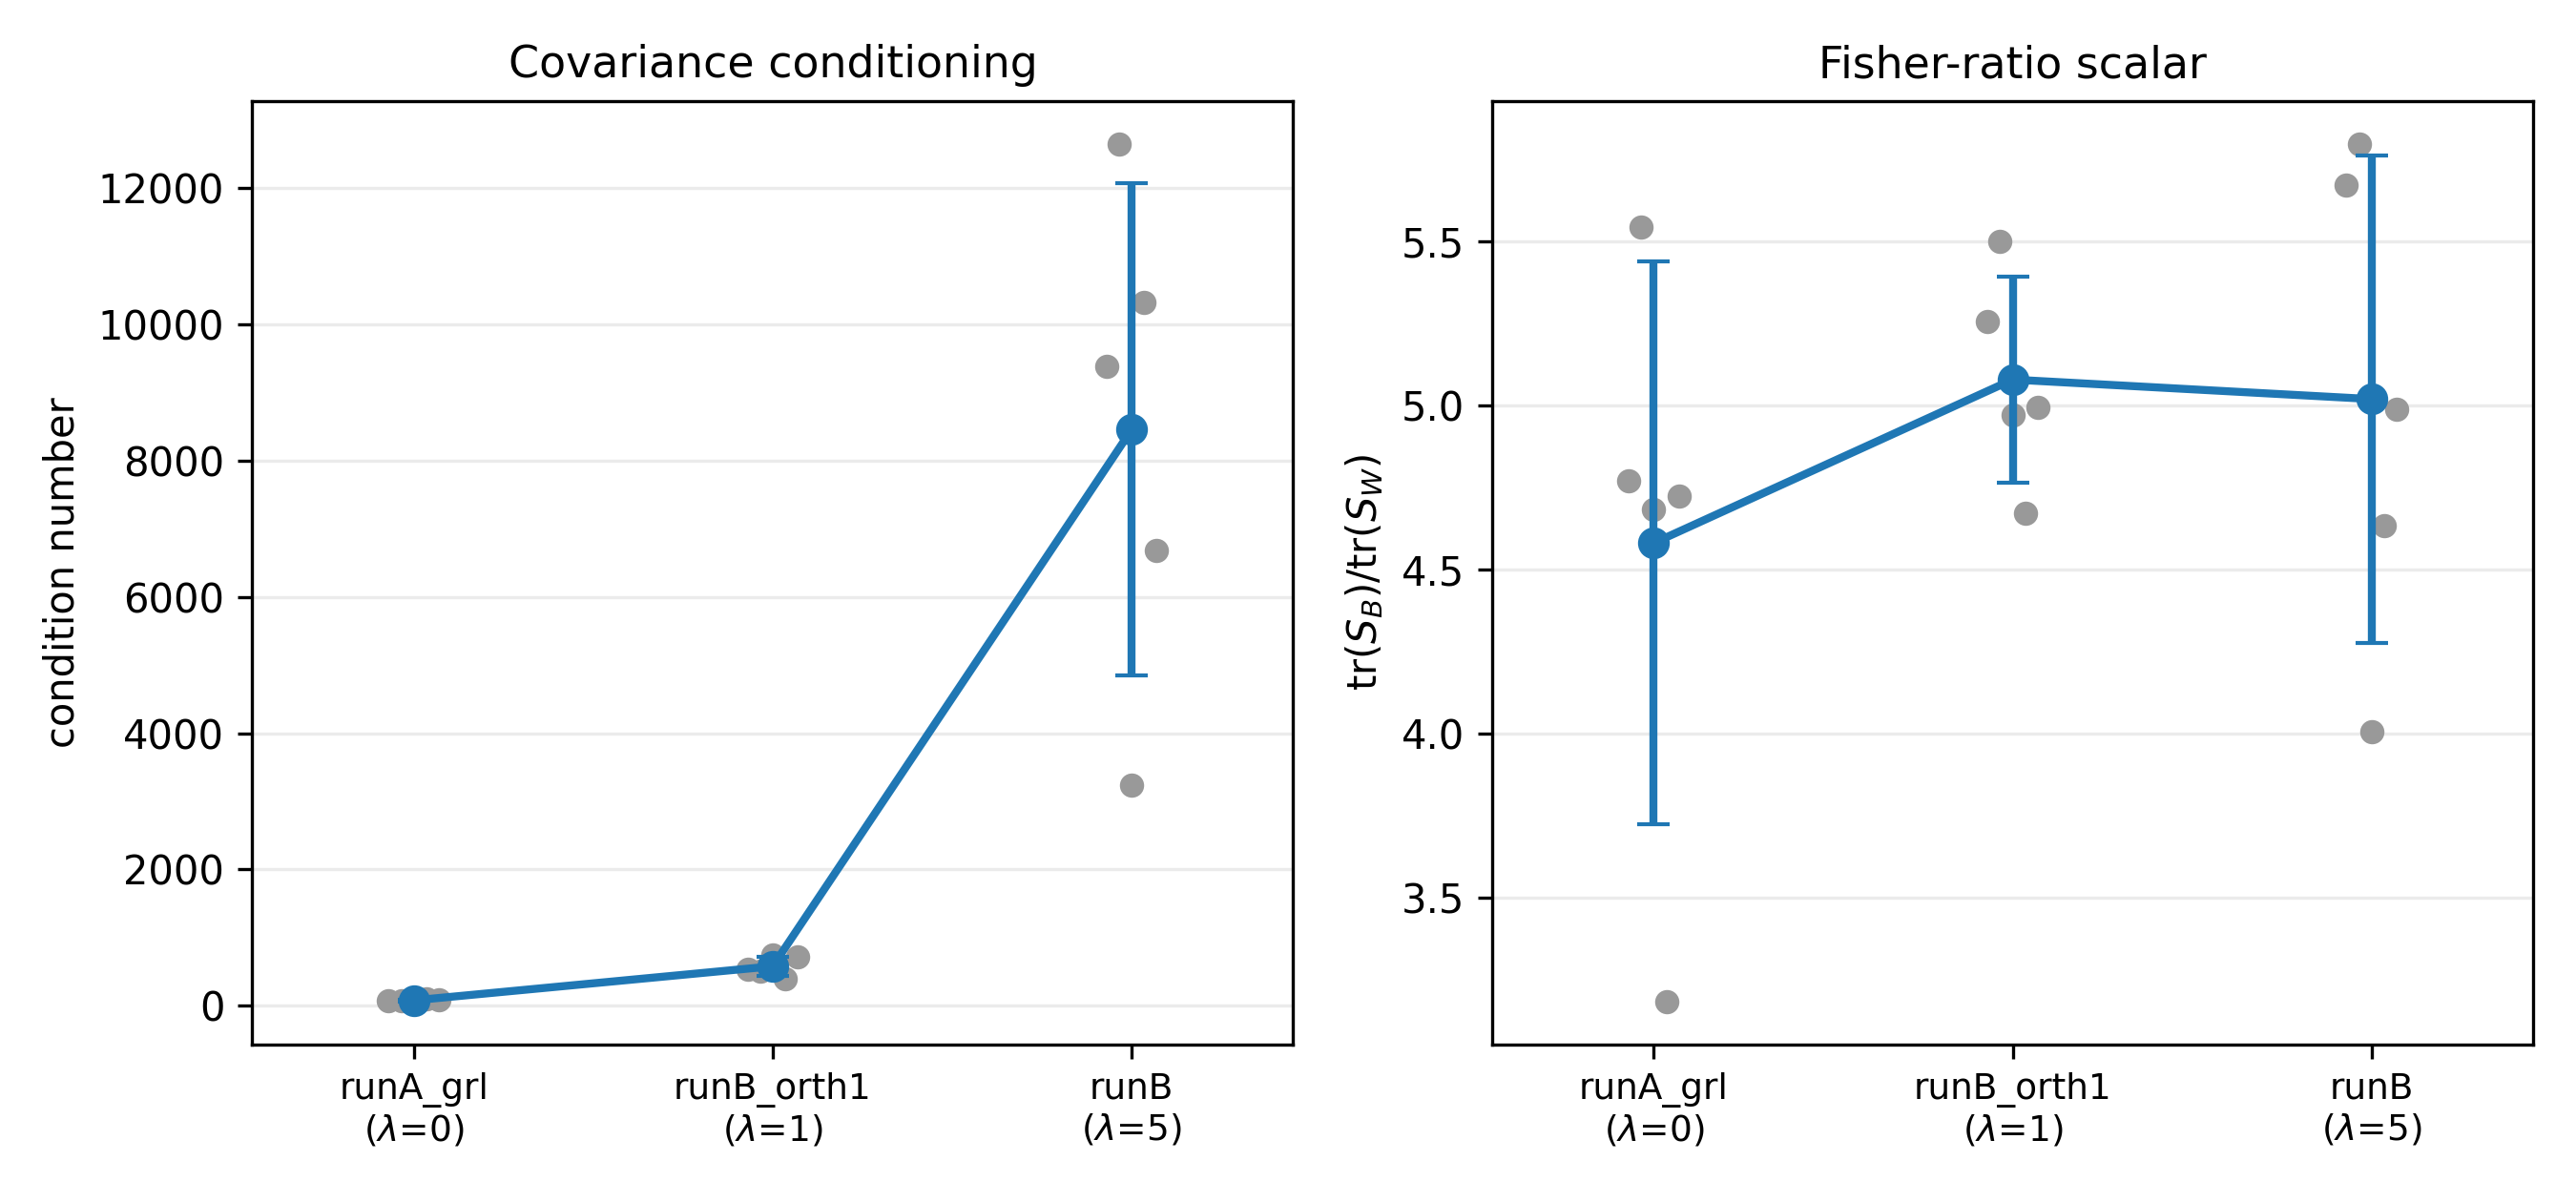
\includegraphics[width=0.62\linewidth]{figs/fig2_geometry_ladder.png}
\caption{Representation geometry across the orthogonality-strength ladder. Condition number (left) and the decoupled Fisher-ratio scalar $\mathrm{tr}(S_B)/\mathrm{tr}(S_W)$ (right) for each of 13 checkpoints (gray points; mean $\pm$ SD in blue), across three levels of orthogonality strength. Condition number increases by approximately two orders of magnitude with $\lambda_{\mathrm{orth}}$ (Kendall's $\tau = 0.84$, exact $p = 2.8 \times 10^{-5}$; Table~\ref{tab:geometry}); the Fisher-ratio scalar shows no significant trend.}
\label{fig:geometry-ladder}
\end{figure}

\subsection{Representation geometry shows no measurable association with Mahalanobis AUROC}
\label{sec:geometry-auroc}

Mahalanobis AUROC (ISIC-test vs.\ PAD-UFES) was $0.401 \pm 0.028$ (\texttt{runA\_grl}), $0.408 \pm 0.022$ (\texttt{runB\_orth1}), and $0.393 \pm 0.025$ (\texttt{runB}) --- below the chance value of 0.5 at every rung (Table~\ref{tab:mahalanobis-auroc} in Appendix~\ref{app:results-extra}).

None of the five geometry metrics, including condition number, showed a significant association with Mahalanobis AUROC: condition number, $\tau = -0.13$, $p = 0.59$; Fisher ratio (HL), $\tau = -0.28$, $p = 0.20$; Fisher ratio (scalar), $\tau = -0.15$, $p = 0.51$; Mardia's kurtosis ($b$), $\tau = -0.13$, $p = 0.59$; Mardia's kurtosis ($z$), $\tau = -0.13$, $p = 0.59$ (Figure~\ref{fig:geometry-vs-auroc}). AUROC itself showed no significant trend across the ladder (Jonckheere--Terpstra, $J = 25.0$, null mean 27.5, exact one-sided $p = 0.65$). Given only $n = 13$ checkpoints these results are inconclusive with respect to small-to-moderate monotonic associations rather than evidence of their absence: at this design no $|\tau|$ below $0.436$ can reach $p \leq 0.05$ under the exact permutation null, and all five bootstrap intervals remain wide enough to contain $|\tau| = 0.3$, the widest admitting $|\tau| = 0.75$ (Section~\ref{sec:power}; Appendix~\ref{app:power}, Table~\ref{tab:tau-ci}).

\begin{quote}
\emph{An approximately two-orders-of-magnitude change in condition number (Section~\ref{sec:geometry-changes}) is not accompanied by a significant change in Mahalanobis AUROC; no geometry metric tested shows a significant association with AUROC.}
\end{quote}

\subsection{Distance-based scores are systematically lower for the target domain}
\label{sec:systematic-lower}

Median Mahalanobis squared distance was lower for PAD-UFES than for ISIC-test at every one of the 13 checkpoints. Pooled across seeds within each rung: \texttt{runA\_grl}, ISIC-test median 13.50 vs.\ PAD-UFES median 8.57 ($n_{\mathrm{id}} = 25335$, $n_{\mathrm{ood}} = 11490$); \texttt{runB\_orth1}, 14.10 vs.\ 8.99 (same $n$); \texttt{runB}, 13.20 vs.\ 8.08 ($n_{\mathrm{id}} = 15201$, $n_{\mathrm{ood}} = 6894$). Two candidate explanations for that gap --- a feature-norm difference between domains, and excess attraction of PAD-UFES samples to the majority ISIC class --- were examined and neither accounts for it on its own; Appendix~\ref{app:results-extra} reports both analyses and Figure~\ref{fig:norm-majority}.

\subsection{Directional misalignment is consistent across three distance-based scorer families}
\label{sec:generalizes}

Pooled across all 13 checkpoints, $\mathrm{AUROC}_{\mathrm{dir}}$ was $0.402 \pm 0.024$ (Mahalanobis), $0.418 \pm 0.022$ (cosine-to-centroid), $0.424 \pm 0.023$ ($k$-NN, $k=1$), $0.414 \pm 0.024$ ($k$-NN, $k=10$), and $0.411 \pm 0.023$ ($k$-NN, $k=50$) (Table~\ref{tab:five-scorers}; Figure~\ref{fig:five-scorers} in Appendix~\ref{app:results-extra}). All five directed values fall within a 0.40--0.42 range, below the chance value of 0.5; the corresponding $\mathrm{AUROC}_{\mathrm{sep}}$ values are 0.576--0.598. The scalar distances therefore retain weak domain-separation signal but consistently order PAD-UFES samples opposite to the scorers' pre-specified OOD semantics. Despite substantially different scoring formulations --- parametric with covariance, parametric without covariance, and non-parametric --- all three families produced highly similar directional misalignment.

None of the five variants showed a significant association with $\lambda_{\mathrm{orth}}$: Mahalanobis, $\tau = -0.08$, $p = 0.80$; cosine, $\tau = 0.32$, $p = 0.19$; $k$-NN ($k=1$), $\tau = -0.05$, $p = 0.90$; $k$-NN ($k=10$), $\tau = 0.02$, $p = 1.00$; $k$-NN ($k=50$), $\tau = 0.08$, $p = 0.80$. Jonckheere--Terpstra gave the same result for all five (exact one-sided $p$ between 0.10 and 0.65; not independent of the Kendall tests, by the identity in Section~\ref{sec:stats}). As in Section~\ref{sec:geometry-auroc}, the small sample leaves these estimates inconclusive with respect to small-to-moderate effects: the critical value on the 5/5/3 ladder is $|\tau| = 0.473$ and all five intervals admit $|\tau| = 0.3$ (Appendix~\ref{app:power}, Table~\ref{tab:tau-ci}). Cosine-to-centroid has the largest point estimate ($\tau = 0.32$, 95\% CI $[-0.21, 0.69]$); it exceeds $0.3$ in magnitude but falls well short of significance at this design, and we do not read it as a trend.

These results do not show that the distance scores are devoid of domain-separation information. All five variants retain weak orientation-free separation and impose it in the direction opposite to their intended operational semantics. Because the reverse orientation is identified using evaluation labels, it is interpreted diagnostically and is not presented as a post-hoc corrected OOD detector.

\begin{quote}
\emph{Three structurally distinct distance-based scorer families report directed AUROC in the same 0.40--0.42 range and orientation-free separability of only 0.58--0.60. The scores are weakly separating but consistently misaligned with the pre-specified higher-distance-is-more-OOD direction; none shows a significant association with $\lambda_{\mathrm{orth}}$.}
\end{quote}

\begin{table}[t]
\centering
\caption{Directed OOD AUROC and orientation-free separability (ISIC-test vs.\ PAD-UFES) for five distance-based scorers (mean $\pm$ SD across seeds). Panel A preserves the pre-specified higher-distance-is-more-OOD direction by rung. Panel B separates this operational result from descriptive, orientation-free scalar separability.}
\label{tab:five-scorers}
\small
\begin{tabular}{lccc}
\toprule
\multicolumn{4}{l}{\textbf{Panel A: $\mathrm{AUROC}_{\mathrm{dir}}$ by ladder rung}} \\
\addlinespace
Scorer & \texttt{runA\_grl} & \texttt{runB\_orth1} & \texttt{runB} \\
\midrule
Mahalanobis & $0.401 \pm 0.028$ & $0.408 \pm 0.022$ & $0.393 \pm 0.025$ \\
Cosine-to-centroid & $0.411 \pm 0.020$ & $0.413 \pm 0.015$ & $0.439 \pm 0.027$ \\
$k$-NN ($k=1$) & $0.424 \pm 0.028$ & $0.428 \pm 0.020$ & $0.416 \pm 0.028$ \\
$k$-NN ($k=10$) & $0.413 \pm 0.029$ & $0.417 \pm 0.020$ & $0.408 \pm 0.029$ \\
$k$-NN ($k=50$) & $0.411 \pm 0.027$ & $0.414 \pm 0.020$ & $0.408 \pm 0.030$ \\
\midrule
\multicolumn{4}{l}{\textbf{Panel B: pooled directional validity vs.\ orientation-free separability ($n=13$)}} \\
\addlinespace
Scorer & $\mathrm{AUROC}_{\mathrm{dir}}$ & $\mathrm{AUROC}_{\mathrm{sep}}$ & Interpretation \\
\midrule
Mahalanobis & $0.402 \pm 0.024$ & $0.598 \pm 0.024$ & reversed, weak \\
Cosine-to-centroid & $0.418 \pm 0.022$ & $0.582 \pm 0.022$ & reversed, weak \\
$k$-NN ($k=1$) & $0.424 \pm 0.023$ & $0.576 \pm 0.023$ & reversed, weak \\
$k$-NN ($k=10$) & $0.414 \pm 0.024$ & $0.586 \pm 0.024$ & reversed, weak \\
$k$-NN ($k=50$) & $0.411 \pm 0.023$ & $0.589 \pm 0.023$ & reversed, weak \\
\bottomrule
\end{tabular}
\end{table}


\subsection{Domain information remains decodable despite directionally misaligned distance scoring}
\label{sec:decodable}

On the identical embeddings scored in Section~\ref{sec:scorers}, three supervised probes recovered domain membership (ISIC-test vs.\ PAD-UFES) at: \texttt{runA\_grl}, 0.719 (logistic regression), 0.717 (linear SVM), 0.807 (random forest); \texttt{runB\_orth1}, 0.741, 0.740, 0.815; \texttt{runB}, 0.750, 0.751, 0.800 (Table~\ref{tab:probe-vs-distance}, Figure~\ref{fig:decodable}). AUROC exceeded 0.70 for all three probe families at every rung. None showed a significant association with $\lambda_{\mathrm{orth}}$ (logistic regression, $\tau = 0.26$, $p = 0.30$; linear SVM, $\tau = 0.26$, $p = 0.30$; random forest, $\tau = -0.11$, $p = 0.70$); these estimates are subject to the same $n = 13$ limitation, and each of the three intervals admits $|\tau| = 0.3$ (Appendix~\ref{app:power}, Table~\ref{tab:tau-ci}).

\begin{quote}
\emph{Three independent classifiers, applied to the same embeddings scored by the distance-based scorers in Section~\ref{sec:scorers}, recover domain membership at 0.72--0.81 AUROC at every $\lambda_{\mathrm{orth}}$ level tested; probe AUROC shows no significant association with $\lambda_{\mathrm{orth}}$.}
\end{quote}

\begin{table}[t]
\centering
\caption{Mean directed distance-scorer AUROC vs.\ domain-probe AUROC, by rung. Directed AUROC is the unweighted mean across the five scorer variants in Table~\ref{tab:five-scorers}. \texttt{baseline\_soft} is a descriptive reference, not a fourth ladder point (Section~\ref{sec:ladder}).}
\label{tab:probe-vs-distance}
\small
\begin{tabular}{llcccc}
\toprule
Rung & Role & Directed AUROC & Probe (LR) & Probe (SVM) & Probe (RF) \\
\midrule
\texttt{runA\_grl} & primary ladder & 0.412 & 0.719 & 0.717 & 0.807 \\
\texttt{runB\_orth1} & primary ladder & 0.414 & 0.741 & 0.740 & 0.815 \\
\texttt{runB} & primary ladder & 0.413 & 0.750 & 0.751 & 0.800 \\
\texttt{baseline\_soft} & categorical reference ($n=1$) & 0.828 & 0.998 & 0.997 & 0.977 \\
\bottomrule
\end{tabular}
\end{table}

\begin{figure}[t]
\centering
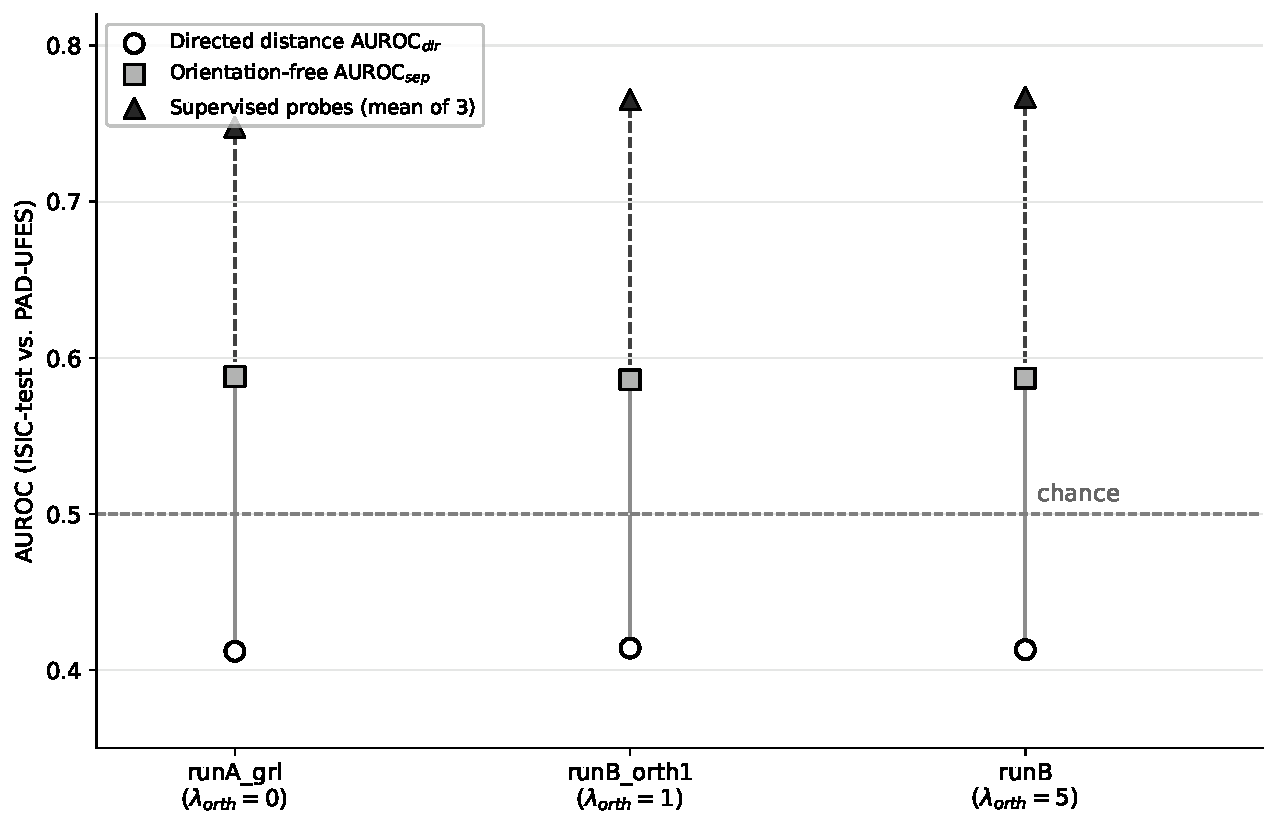
\includegraphics[width=0.62\linewidth]{figs/fig6_directional_misalignment.pdf}
\caption{Domain decodability exceeds both directed distance ranking and orientation-free scalar separability. For each rung, the mean directed AUROC across five distance scorers (open circles) is linked to its orientation-free counterpart, $1-\mathrm{AUROC}_{\mathrm{dir}}$ in this below-chance regime (gray squares), and to mean AUROC across three supervised domain probes (black triangles). Directed distance ranking remains near 0.41, orientation-free separability near 0.59, and supervised probe AUROC near 0.75--0.77. Solid segments mark the score-orientation gap; dashed segments mark the remaining gap between scalar distance separability and supervised decodability from the full embedding. Orientation-free values are diagnostic and do not represent a detector whose polarity was calibrated on independent data.}
\label{fig:decodable}
\end{figure}

\subsection{Descriptive reference: a conventional non-adversarial baseline}
\label{sec:baseline-reference}

For a single ResNet-50 checkpoint (\texttt{baseline\_soft}; one seed, architecture and representation dimensionality differing from the ladder, Section~\ref{sec:ladder}), pooled distance-scorer AUROC was 0.828 and probe AUROC was 0.998 (logistic regression), 0.997 (linear SVM), and 0.977 (random forest) (Table~\ref{tab:probe-vs-distance}).

\section{Discussion}
\label{sec:discussion}

\subsection{Interpretation}
\label{sec:interpretation}

The results support a three-level interpretation that separates operational validity, scalar-score information, and information recoverable from the full embedding.

\paragraph{Level 1: the pre-specified operational direction fails.}
All five distance-score variants produced $\mathrm{AUROC}_{\mathrm{dir}}=0.402$--$0.424$ under the higher-distance-is-more-OOD convention (Section~\ref{sec:generalizes}), ranking PAD-UFES samples as more source-typical than ISIC-test samples. This is an operational polarity failure: a reliability gate using the direction specified before evaluation would rank the audited target domain incorrectly. Agreement across Mahalanobis, cosine-to-centroid, and pooled $k$-NN shows the pattern is not confined to covariance inversion or to one value of $k$.

\paragraph{Level 2: the scalar scores retain weak separation signal.}
A directed AUROC below 0.5 does not imply absence of information. Removing orientation yields $\mathrm{AUROC}_{\mathrm{sep}}=0.576$--$0.598$, so the distances weakly separate the two domains while ordering them opposite to the intended semantics --- neither chance-level non-separation nor a valid detector obtained by negation. The reverse orientation was identified from evaluation labels; without polarity selection on independent calibration data, $\mathrm{AUROC}_{\mathrm{sep}}$ remains diagnostic rather than deployable performance.

\paragraph{Level 3: the full embeddings support stronger supervised decodability.}
Probes recovered domain membership at 0.72--0.81 AUROC from the same embeddings (Section~\ref{sec:decodable}). Figure~\ref{fig:decodable} therefore exposes two distinct gaps: between the intended and observed direction of the scalar scores, and between their weak orientation-free separability and the stronger decodability available from the full representation. Probe success is an existence test only; it does not imply that the original classifier or any unsupervised reliability mechanism uses the decoded information.

This also constrains the geometry result. Covariance conditioning moved by approximately two orders of magnitude (Section~\ref{sec:geometry-changes}), but neither directed Mahalanobis AUROC nor the other scorer families tracked that change. The conclusion is not that geometry is irrelevant, but that condition number alone is insufficient to predict either the direction or the strength of the rank ordering these source-fitted scores induce. Section~\ref{sec:systematic-lower} confirms a systematic distance-ordering difference without fully explaining its origin; establishing why the targeted domain is ranked as source-typical remains future work. The supported claim is therefore scoped: within this domain-adversarial regime and for its adversarial target domain, the tested source-fitted distance rules are directionally misaligned, their scalar outputs retain weak separation, and the full embeddings retain stronger supervised domain decodability. This is not a claim that scalar distances contain no information, that supervised probes constitute an OOD detector, or that domain-adversarial training or orthogonality regularization causes the observed ordering.

\subsection{Scorer-relevant geometry}
\label{sec:invariance-pointer}

Part of why a large conditioning change need not move AUROC is structural rather than empirical: for a full-rank affine change of coordinates the unregularized squared Mahalanobis distance is invariant while the condition number $\kappa(\Sigma)$ can change by orders of magnitude, and cosine-to-centroid, $k$-NN, and AUROC itself each preserve a different set of transformations. The chain from raw geometric change to score change to ranking change to AUROC change is therefore not automatic, and ``geometry'' is not one object for this purpose. Appendix~\ref{app:invariance} develops this argument, states each scorer's invariances, and draws out the audit principle that follows: evaluation should separately test score polarity, orientation-free separation, and information recoverable from the representation, while identifying the invariances of the downstream scorer.

\subsection{Relation to literature}
\label{sec:relation-lit}

Mahalanobis-distance OOD detection \citep{lee2018simple} and its non-parametric successors, including pooled $k$-nearest-neighbor scoring \citep{sun2022knn}, are typically evaluated by benchmarking AUROC across datasets and architectures, not by separately auditing score polarity, orientation-free separability, and full-embedding decodability after a representation-changing intervention. This study proposes no competitor to either; both are used as audit instruments, alongside cosine-to-centroid scoring. Their common result here is a shared directional misalignment with weak residual separation --- not a comparative ranking and not evidence that their scalar outputs contain no information.

Domain-adversarial representation learning \citep{ganin2015unsupervised, ganin2016domain} and orthogonality-based shared/private separation \citep{bousmalis2016domain} are among the strategies proposed to reduce reliance on nuisance or shortcut features \citep{geirhos2020shortcut}. This study does not identify that training family as the cause of the observed ordering, because every ladder checkpoint already uses the domain-adversarial regime and the conventional baseline is not matched. It asks instead whether source-fitted distance scores retain their intended polarity and how much separation survives when orientation is ignored; for the audited target domain the intended polarity fails and residual separability is weak, while causal attribution to domain-adversarial training, orthogonality regularization, architecture, or dimensionality remains outside the evidence provided here. Appendix~\ref{app:relation-lit} extends this to the probing and geometry--performance literatures and to the practitioner implications.

\subsection{Limitations}
\label{sec:limitations}

PAD-UFES is not an arbitrary target domain: it is the domain the architecture's adversarial branch is trained against. Our conclusions therefore characterize representations learned under this training regime, not all domain shifts.

$\mathrm{AUROC}_{\mathrm{sep}}$ is computed from the observed evaluation ordering and is reported only as an orientation-free diagnostic. This study includes no independent calibration split on which score polarity could be selected and then transferred unchanged to a held-out target. It therefore does not establish that negating a distance score yields an operational detector, that the reverse polarity transfers to another shift, or that a deployed system could identify the required polarity without labeled shifted data.

The conventional non-adversarial baseline (Section~\ref{sec:baseline-reference}) differs from the ladder in architecture, representation dimensionality, and training recipe simultaneously, and is a single checkpoint. It is descriptive and supports no causal attribution of the ladder findings to domain-adversarial training or orthogonality regularization as opposed to architecture or dimensionality; a matched non-adversarial checkpoint at the same architecture and 16-dimensional representation would be needed, and none exists in the available inventory.

The ladder spans three ordinal levels with unequal seed counts ($n = 13$; $n = 9$ on the common-seed subset). The exact critical values are $0.436$, $0.473$, and $0.609$, while power at an expected $\tau = 0.3$ is only $0.27$, $0.23$, and $0.14$ (Appendix~\ref{app:power}). The combined analysis criterion --- $|\tau| \geq 0.3$ and $p \leq 0.05$ --- could therefore not be satisfied by an association of exactly that magnitude at any of the three designs, and none of the seventeen non-significant intervals excludes a moderate association of magnitude $0.3$ in at least one direction. The consistent point-estimate pattern bounds but does not eliminate uncertainty about whether $\lambda_{\mathrm{orth}}$ modulates the observed misalignment; the tests are also correlated, reusing metrics, scorers, and probes derived from the same embeddings. Exact-permutation testing was used throughout in place of unverified asymptotic approximations, and $p$-values carry no family-wise correction; a reader applying a stricter correction should note that the one large, load-bearing effect --- condition number against $\lambda_{\mathrm{orth}}$, $\tau = 0.840$, the design maximum --- survives any standard correction, while every non-significant result was reported as such before any correction was considered.

This study includes no replication on a domain independent of the ISIC/PAD-UFES pair and no check of generalization beyond the single audited architecture. Both were considered and omitted: a third-domain replication needs a dataset without documented image overlap with the training data, which was unavailable within scope, and the cross-architecture check was not pursued for the same reason. Neither gap is filled by the baseline reference, which addresses architecture and dimensionality but not domain independence. The bootstrap check that would quantify shared estimation noise between condition number and Fisher ratio, both derived from the same fitted precision matrix, was not performed; condition number, not Fisher ratio, drives the geometric finding in Section~\ref{sec:geometry-changes}, which bounds but does not remove this uncertainty. Mardia's kurtosis null was calibrated with 200 bootstrap resamples per checkpoint; the regularization constant ($\varepsilon = 10^{-5}$) and the 16-dimensional representation were inherited from the audited classifier rather than varied here. ``Reliability estimation'' throughout means out-of-distribution detection AUROC specifically; calibration \citep{guo2017calibration} and selective prediction, including distribution-free variants \citep{elyaniv2010foundations, geifman2017selective, angelopoulos2023conformal}, are not addressed.

These limitations reinforce the three-level interpretation: the pre-specified operational direction is invalid for the audited target domain, the scalar scores retain weak orientation-free separation, and the full embeddings support stronger supervised decodability. None of these observations alone establishes transfer to an unseen domain or the performance of a calibrated deployment system.

\section{Conclusion}
\label{sec:conclusion}

This study audited the relationship among measured representation structure, distance-based OOD ordering, scalar separability, and supervised domain decodability within a fixed domain-adversarial training regime. Across an orthogonality-strength ladder, covariance conditioning changed by approximately two orders of magnitude while the other four geometry summaries showed no significant ladder trend, and that geometric change was not accompanied by a corresponding change in Mahalanobis OOD ranking or in any other tested distance-score family.

Under the pre-specified higher-distance-is-more-OOD convention, five variants from three scorer families produced $\mathrm{AUROC}_{\mathrm{dir}}=0.402$--$0.424$. These scores were not devoid of domain-separation information: ignoring orientation yields $\mathrm{AUROC}_{\mathrm{sep}}=0.576$--$0.598$. The information encoded in the scalar distances was therefore weak and systematically ordered opposite to the intended OOD semantics; because that reverse orientation was identified from evaluation labels, it is a diagnostic finding rather than an operationally corrected detector. Supervised probes on the full embeddings recovered substantially stronger domain membership information at 0.72--0.81 AUROC.

The supported conclusion is narrower and more precise than either complete distance inaccessibility or a causal claim about disentanglement: within the audited representations, domain membership remains decodable, scalar distance scores retain weak separation, and the tested source-fitted distance rules impose a directionally misaligned OOD ordering. Raw geometric summaries, scorer-relevant geometry, score orientation, orientation-free separability, and supervised decodability should be treated as distinct objects of evaluation. Reliability mechanisms layered on learned representations should be re-validated after representation-changing interventions --- including explicit validation of score polarity on data independent of the final evaluation set --- rather than assumed to inherit validity from classification performance or generic geometric diagnostics.

\section*{Broader Impact Statement}
\label{sec:broader-impact}

This study is a retrospective, methodological audit conducted entirely on two pre-existing, publicly available, de-identified skin-lesion image datasets. It trains no new diagnostic classifier, deploys no system, and releases no model intended for clinical use; the audited checkpoints form an orthogonality-strength ladder within a domain-adversarial regime for the purpose of this analysis. No patients were recruited and no new clinical images were acquired.

The central risk this work is positioned to mitigate, rather than create, is the silent failure of a distance-based reliability safeguard in a deployed pipeline: if such a safeguard is assumed to function on representations produced by a domain-adversarial training regime, without being re-validated against the domain targeted during training, it may fail to flag inputs from precisely that domain. Making this failure mode explicit and measurable is intended to reduce, not increase, the risk of over-trusting a distance-based safeguard in a safety-critical medical imaging pipeline. We are not aware of a plausible negative use of this study's findings or artifacts: the audit protocol, the geometry metrics, and the statistical tests reported here characterize an existing training regime rather than introduce a new capability that could be misapplied. We therefore do not identify a significant risk of harm requiring further mitigation beyond the cautions already stated in Section~\ref{sec:limitations} regarding the scope of the claims.


\bibliography{references}
\bibliographystyle{tmlr}

\appendix

\section{Detectability, power, and interval estimates}
\label{app:power}

This appendix reports the three quantities defined in Section~\ref{sec:power}
for every association tested in this paper. All of them are computed from the
per-checkpoint results already reported in Section~\ref{sec:results}: no
checkpoint is re-evaluated, no model is retrained, and no additional data are
used.

\subsection{What the designs could have detected}
\label{app:power-design}

Two permutation designs are used in this paper and they are not
interchangeable. Design~A is continuous--continuous (a geometry metric against
Mahalanobis AUROC, $n = 13$, tie-free), and its exact null runs over all $13!$
orderings. Design~B tests an ordinal dose against a value (a geometry metric,
scorer AUROC, or probe AUROC against $\lambda_{\mathrm{orth}}$), where the dose
is tied by construction and the exact null runs over the $72{,}072$ distinct
label arrangements consistent with the 5/5/3 rung counts, or the $1{,}680$
arrangements of the 3/3/3 common-seed subset. Table~\ref{tab:power-design}
gives $\tau_{\mathrm{crit}}$, the attainable maximum $|\tau|$, and power for
each; Figure~\ref{fig:power}(A) shows the full power curves.

Design~B's attainable maximum is $0.840$ rather than $1.000$ because a tied
predictor caps $\tau_b$ below unity: with 5/5/3 rung sizes, a perfectly
monotone ladder --- every checkpoint at a lower $\lambda_{\mathrm{orth}}$
ranked below every checkpoint at a higher one --- yields exactly $\tau_b =
0.840$. The condition-number result of Section~\ref{sec:geometry-changes}
attains that ceiling.

% generated by analysis/make_tables_power_tmlr.py from
% results/power_design_summary.csv -- do not edit by hand.
\begin{table}[t]
\centering
\caption{Detectability of the two permutation designs used in this study.
Design~A is the continuous--continuous test of a geometry metric against
Mahalanobis AUROC (Section~\ref{sec:geometry-auroc}); Design~B is the ordered
ladder used for every test against $\lambda_{\mathrm{orth}}$
(Sections~\ref{sec:geometry-changes}, \ref{sec:generalizes} and
\ref{sec:decodable}). ``Null space'' is the number of distinct label
arrangements enumerated for the exact test.
$\tau_{\mathrm{crit}}$ is the smallest $|\tau|$ attainable at that design whose
two-sided exact permutation $p$-value reaches $0.05$: no dataset, however clean,
can produce a significant association below it. Power is computed by simulation
($2\times10^{4}$ datasets per grid point, common random numbers) under an
alternative whose expected value of the reported statistic equals the stated
$\tau$ --- bivariate normal for Design~A, a linear dose shift
$y = \theta d + \varepsilon$ for Design~B. MDE$_{80\%}$ is the expected $\tau$ at
which power first reaches $0.80$.}
\label{tab:power-design}
\footnotesize
\begin{tabular}{lccccccc}
\toprule
 & & Null & Max. & & \multicolumn{2}{c}{Power at} & \\
\cmidrule(lr){6-7}
Design & $n$ & space & $|\tau|$ & $\tau_{\mathrm{crit}}$ & $\tau=0.3$ & $\tau=0.5$ & MDE$_{80\%}$ \\
\midrule
A: continuous--continuous & 13 & $13!$ & 1.000 & 0.436 & 0.27 & 0.71 & 0.54 \\
B: 5/5/3 ordered ladder & 13 & 72,072 & 0.840 & 0.473 & 0.23 & 0.63 & 0.57 \\
B: 3/3/3 common-seed subset & 9 & 1,680 & 0.866 & 0.609 & 0.14 & 0.39 & 0.69 \\
\bottomrule
\end{tabular}
\end{table}


\subsection{What the data exclude}
\label{app:power-ci}

Table~\ref{tab:tau-ci} gives a 95\% bias-corrected and accelerated (BCa)
bootstrap interval \citep{efron1987better} for every $\tau$ reported in the
paper, over $2\times10^{4}$ resamples drawn \emph{within} rung so that the
5/5/3 design is held fixed; $\lambda_{\mathrm{orth}}$ is a fixed design factor,
not a sampled one, and resampling across rungs would bootstrap a quantity this
experiment never estimated. Figure~\ref{fig:power}(B) plots the same intervals
against the two designs' critical values.

Resampling with replacement necessarily creates ties in a response that was
tie-free as observed, and the two standard tie treatments pull an interval in
opposite directions: the $\tau_b$ denominator $\sqrt{(n_0 - t_x)(n_0 - t_y)}$
shrinks as ties accumulate and so inflates $|\tau|$ on tied resamples, whereas
the design-normalized form $(2J - M)/\sqrt{M n_0}$ pins the denominator to the
original design and cannot exceed the design ceiling. The two are identical on
the observed data. Both were computed; over the tests reported here their endpoints
differ by a median of $0.027$ and at most $0.091$, and the two agree on every
$|\tau| = 0.3$ exclusion verdict, so no statement in this paper depends on the
choice. Table~\ref{tab:tau-ci}
reports the $\tau_b$ version.

One case admits no valid interval. Where an observed $\tau$ attains the maximum
its design permits --- condition number against $\lambda_{\mathrm{orth}}$,
$\tau = 0.840$ --- every resample lies at or below the observed value, the
resampling distribution is one-sided by construction, and a nominal interval
computed from it can fail even to contain its own point estimate. That case is
reported as a point without an interval, and its exact permutation $p$-value is
the meaningful inference.

% generated by analysis/make_tables_power_tmlr.py from
% results/kendall_tau_ci.csv -- do not edit by hand.
\begin{table}[t]
\centering
\caption{Every Kendall's $\tau$ reported in this paper with a 95\% bootstrap
confidence interval ($2\times10^{4}$ stratified resamples, bias-corrected and
accelerated; resampling is within-rung, so the 5/5/5 design is held fixed).
``Largest $|\tau|$ not excluded'' is the interval endpoint furthest from zero:
the effect size each non-significant result still permits.}
\label{tab:tau-ci}
\small
\begin{tabular}{lccc}
\toprule
Test & $\tau$ & 95\% CI & Largest $|\tau|$ not excluded \\
\midrule
\multicolumn{4}{l}{\emph{Geometry metric vs.\ $\lambda_{\mathrm{orth}}$ (Section~\ref{sec:geometry-changes})}} \\
\addlinespace[0.15em]
\quad Condition number & $\phantom{-}0.845$ & \multicolumn{2}{c}{at design ceiling --- see note} \\
\quad Fisher ratio (Hotelling--Lawley) & $\phantom{-}0.237$ & $[-0.335,\ \phantom{-}0.612]$ & 0.61 \\
\quad Fisher ratio (decoupled scalar) & $\phantom{-}0.237$ & $[-0.313,\ \phantom{-}0.612]$ & 0.61 \\
\quad Mardia's kurtosis ($b$) & $\phantom{-}0.056$ & $[-0.313,\ \phantom{-}0.385]$ & 0.38 \\
\quad Mardia's kurtosis ($z$) & $\phantom{-}0.011$ & $[-0.344,\ \phantom{-}0.363]$ & 0.36 \\
\addlinespace
\multicolumn{4}{l}{\emph{Geometry metric vs.\ Mahalanobis AUROC (Section~\ref{sec:geometry-auroc})}} \\
\addlinespace[0.15em]
\quad Condition number & $\phantom{-}0.143$ & $[-0.253,\ \phantom{-}0.440]$ & 0.44 \\
\quad Fisher ratio (Hotelling--Lawley) & $-0.276$ & $[-0.663,\ \phantom{-}0.216]$ & 0.66 \\
\quad Fisher ratio (decoupled scalar) & $-0.219$ & $[-0.629,\ \phantom{-}0.286]$ & 0.63 \\
\quad Mardia's kurtosis ($b$) & $-0.086$ & $[-0.490,\ \phantom{-}0.339]$ & 0.49 \\
\quad Mardia's kurtosis ($z$) & $-0.067$ & $[-0.460,\ \phantom{-}0.329]$ & 0.46 \\
\addlinespace
\multicolumn{4}{l}{\emph{Directed scorer AUROC vs.\ $\lambda_{\mathrm{orth}}$ (Section~\ref{sec:generalizes})}} \\
\addlinespace[0.15em]
\quad Mahalanobis & $\phantom{-}0.192$ & $[-0.311,\ \phantom{-}0.572]$ & 0.57 \\
\quad Cosine-to-centroid & $\phantom{-}0.372$ & $[-0.151,\ \phantom{-}0.685]$ & 0.68 \\
\quad $k$-NN ($k=1$) & $\phantom{-}0.146$ & $[-0.391,\ \phantom{-}0.589]$ & 0.59 \\
\quad $k$-NN ($k=10$) & $\phantom{-}0.214$ & $[-0.358,\ \phantom{-}0.611]$ & 0.61 \\
\quad $k$-NN ($k=50$) & $\phantom{-}0.304$ & $[-0.192,\ \phantom{-}0.658]$ & 0.66 \\
\addlinespace
\multicolumn{4}{l}{\emph{Domain-probe AUROC vs.\ $\lambda_{\mathrm{orth}}$ (Section~\ref{sec:decodable})}} \\
\addlinespace[0.15em]
\quad Logistic regression & $\phantom{-}0.259$ & $[-0.199,\ \phantom{-}0.612]$ & 0.61 \\
\quad Linear SVM & $\phantom{-}0.304$ & $[-0.152,\ \phantom{-}0.621]$ & 0.62 \\
\quad Random forest & $\phantom{-}0.192$ & $[-0.315,\ \phantom{-}0.543]$ & 0.54 \\
\bottomrule
\end{tabular}

\vspace{0.25cm}
\begin{minipage}{\textwidth}
% undo the \centering of the enclosing table, so the note sets as a paragraph
\leftskip=0pt \rightskip=0pt \parfillskip=0pt plus 1fil
\small \emph{Note.} Condition number vs.\ $\lambda_{\mathrm{orth}}$ attains
$\tau = 0.845$, the maximum value the 5/5/5 design permits (a perfectly monotone
ladder). Every bootstrap resample therefore lies at or below the observed value,
the resampling distribution is one-sided by construction, and no bootstrap
interval is valid; the exact permutation $p$-value ($p = 2.6 \times 10^{-6}$) is the
meaningful inference for that effect. Of the seventeen non-significant
associations, none has an interval that excludes $|\tau| = 0.3$.
\end{minipage}
\end{table}


\begin{figure}[t]
\centering
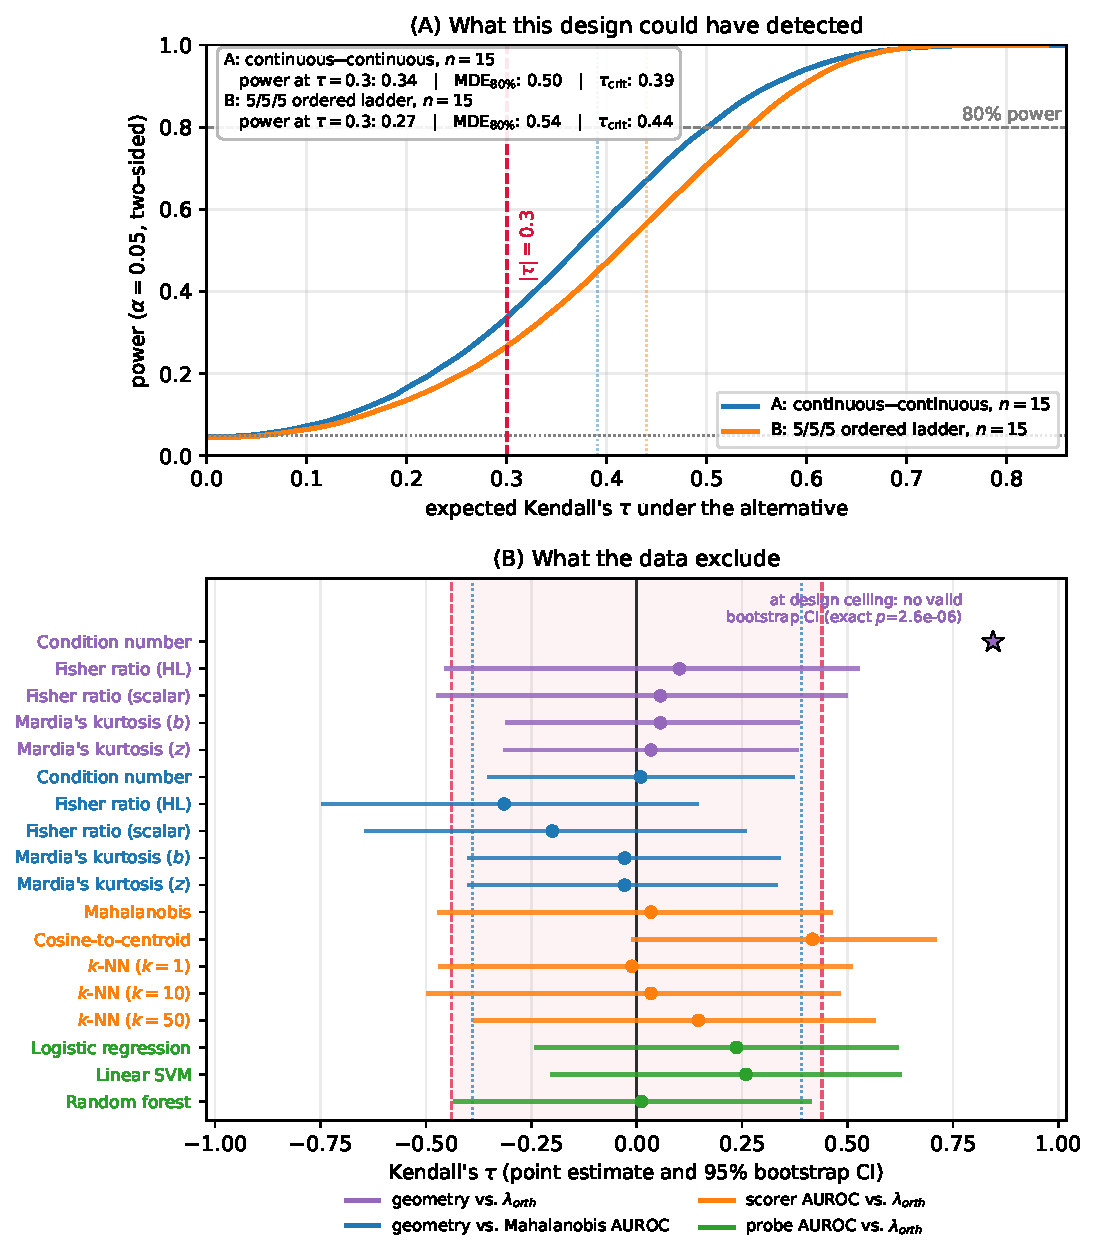
\includegraphics[width=0.93\linewidth]{figs/fig7_power.pdf}
\caption{Effect-size and power bounds on this study's non-significant
associations (exact permutation tests, $\alpha = 0.05$). (A) Power against the
expected value of the reported statistic, for the three designs of
Table~\ref{tab:power-design}; vertical dotted lines mark each design's
$\tau_{\mathrm{crit}}$ and the dashed red line marks $|\tau| = 0.3$, the effect
size fixed in the analysis plan (Section~\ref{sec:stats}). That value lies below
every $\tau_{\mathrm{crit}}$, so the plan's conjunction of $|\tau| \geq 0.3$
with significance at $\alpha = 0.05$ was unsatisfiable at these designs.
(B) Observed Kendall's $\tau$ with 95\% BCa bootstrap intervals for all
eighteen association tests reported in the paper. The shaded band spans
$\pm\tau_{\mathrm{crit}}$ for the 5/5/3 ladder (dashed bounds); dotted bounds
mark the continuous--continuous design. Condition number against
$\lambda_{\mathrm{orth}}$ (star) sits at its design ceiling and is drawn without
an interval, for the reason given in Section~\ref{app:power-ci}.}
\label{fig:power}
\end{figure}


\end{document}
